\documentclass{article} 

\usepackage{graphicx}
\usepackage{booktabs}

\title{Captions and floats}
\author{V Knight}
\date{\today}

\begin{document} 

\maketitle

Figure~\ref{my_picture} shows a cat.

\begin{figure}[!htbp]
    \begin{center}
        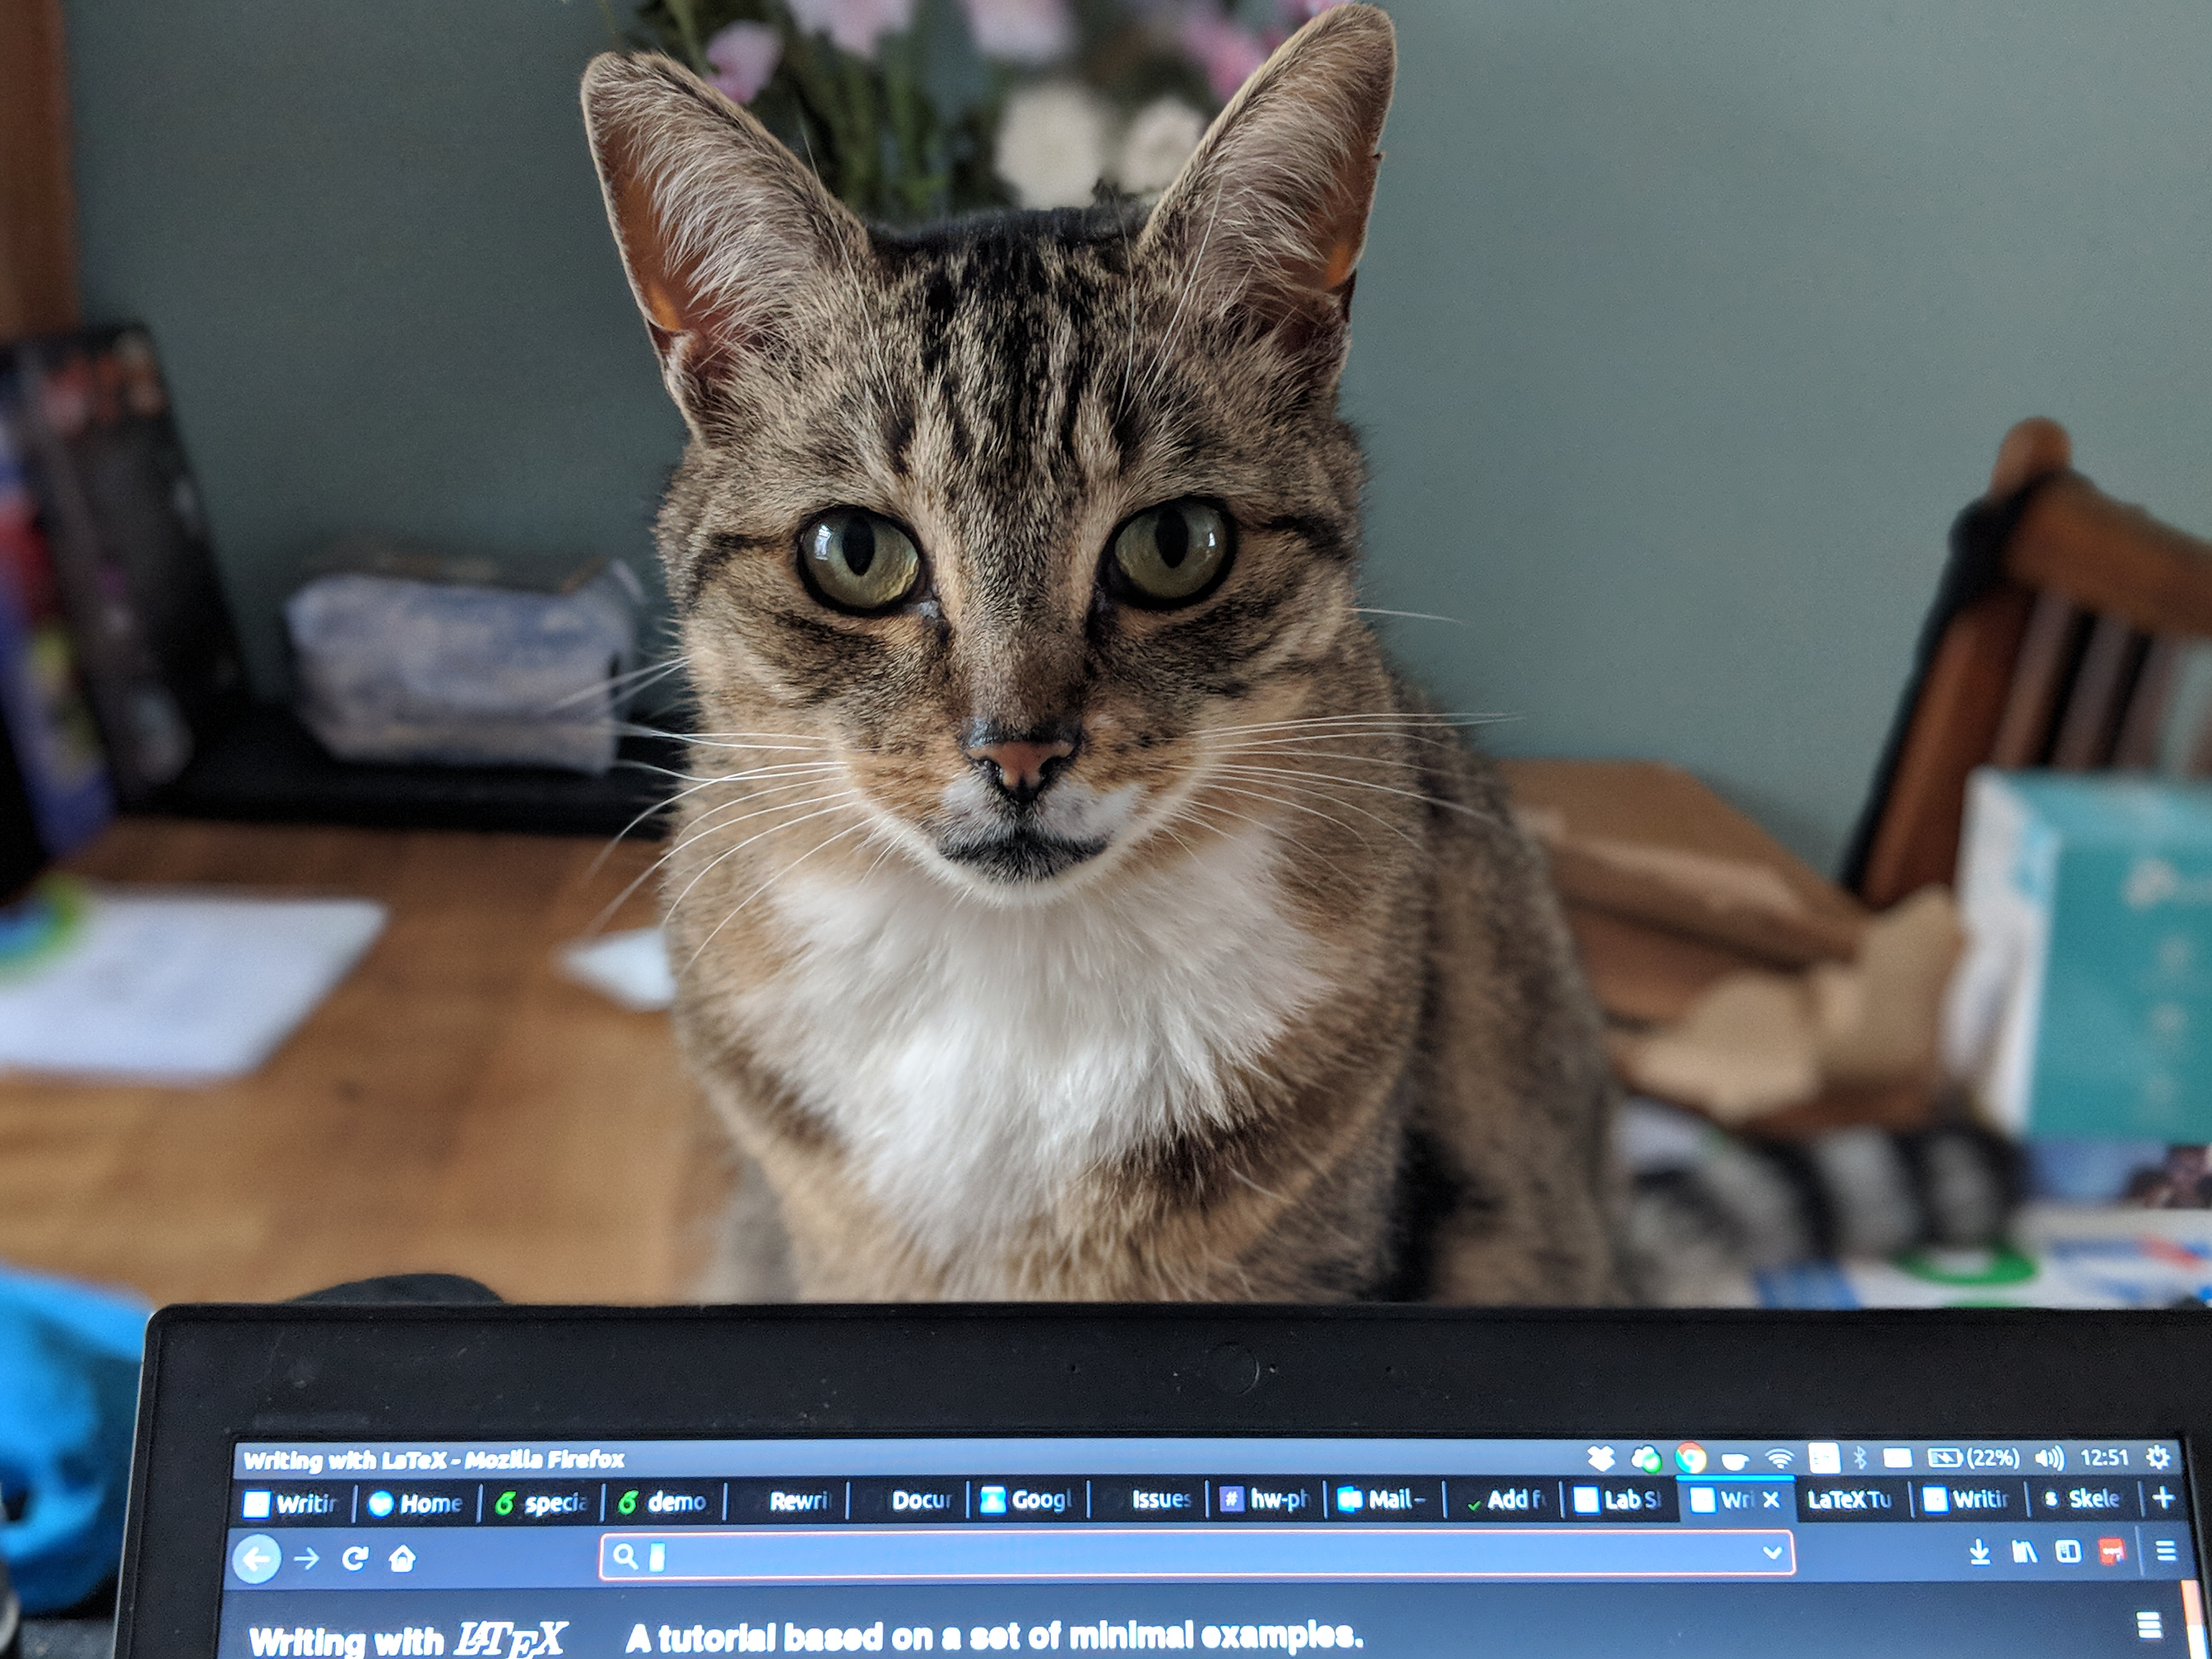
\includegraphics[width=.6\textwidth]{cat.jpg}
    \end{center}
    \caption{A cat}
    \label{my_picture}
\end{figure}

Table~\ref{my_table} shows a table.

\begin{table}[!hbtp]
    \begin{center}
        \begin{tabular}{|l|c|}
            \toprule
            Name    & Animal \\
            \midrule
            Auraya  & dog \\
            Chick   & cat \\
            Duck    & cat \\
            Riggins & dog \\
            \bottomrule
        \end{tabular}
    \end{center}
    \caption{A table of pets}
    \label{my_table}
\end{table}

\end{document}
